\chapter{Instrument Overview}
\label{ch:instruments}

We are in the age of precision cosmology, and measurements of the CMB spectra continue to improve in sensitivity.  Now, to measure the CMB polarization anisotropies, scientists are pushing forward the sensitivity of the instruments by increasing detector numbers, improving detector sensitivity, and controlling optical systematics, to name a few.  For example, the Atacama Cosmology Telescope (ACT), a ground-based cosmology experiment, used roughly 3000 bolometric detectors.  The Simons Observatory is scaling its detector count up to more than 50,000 bolometric detectors in order to improve mapping speed and sensitivity.  Looking ahead, the CMB-S4 collaboration, a next-generation cosmology project, plans to scale up even further: to roughly 500,000 detectors.  This, along with the many other improvements in instrumentation, aim to detect the faintest signals of the CMB polarization spectra.

In this chapter, I describe two ground-based cosmology experiments covered in this work: the Atacama Cosmology Telescope (ACT), an operational cosmology experiment~\cite{act_inst}, and the Simons Observatory (SO), this generation's cutting-edge cosmology experiment~\cite{so19}.  I describe the Simons Observatory Large Aperture Telescope instrument further in Chapters~\ref{ch:mma},~\ref{ch:ot_holo}, and ~\ref{ch:holosim}, and the Small Aperture Telescope in Chapter~\ref{ch:sat_holo}.

\section{Atacama Cosmology Telescope}

\begin{figure*}[t]
    \centering
    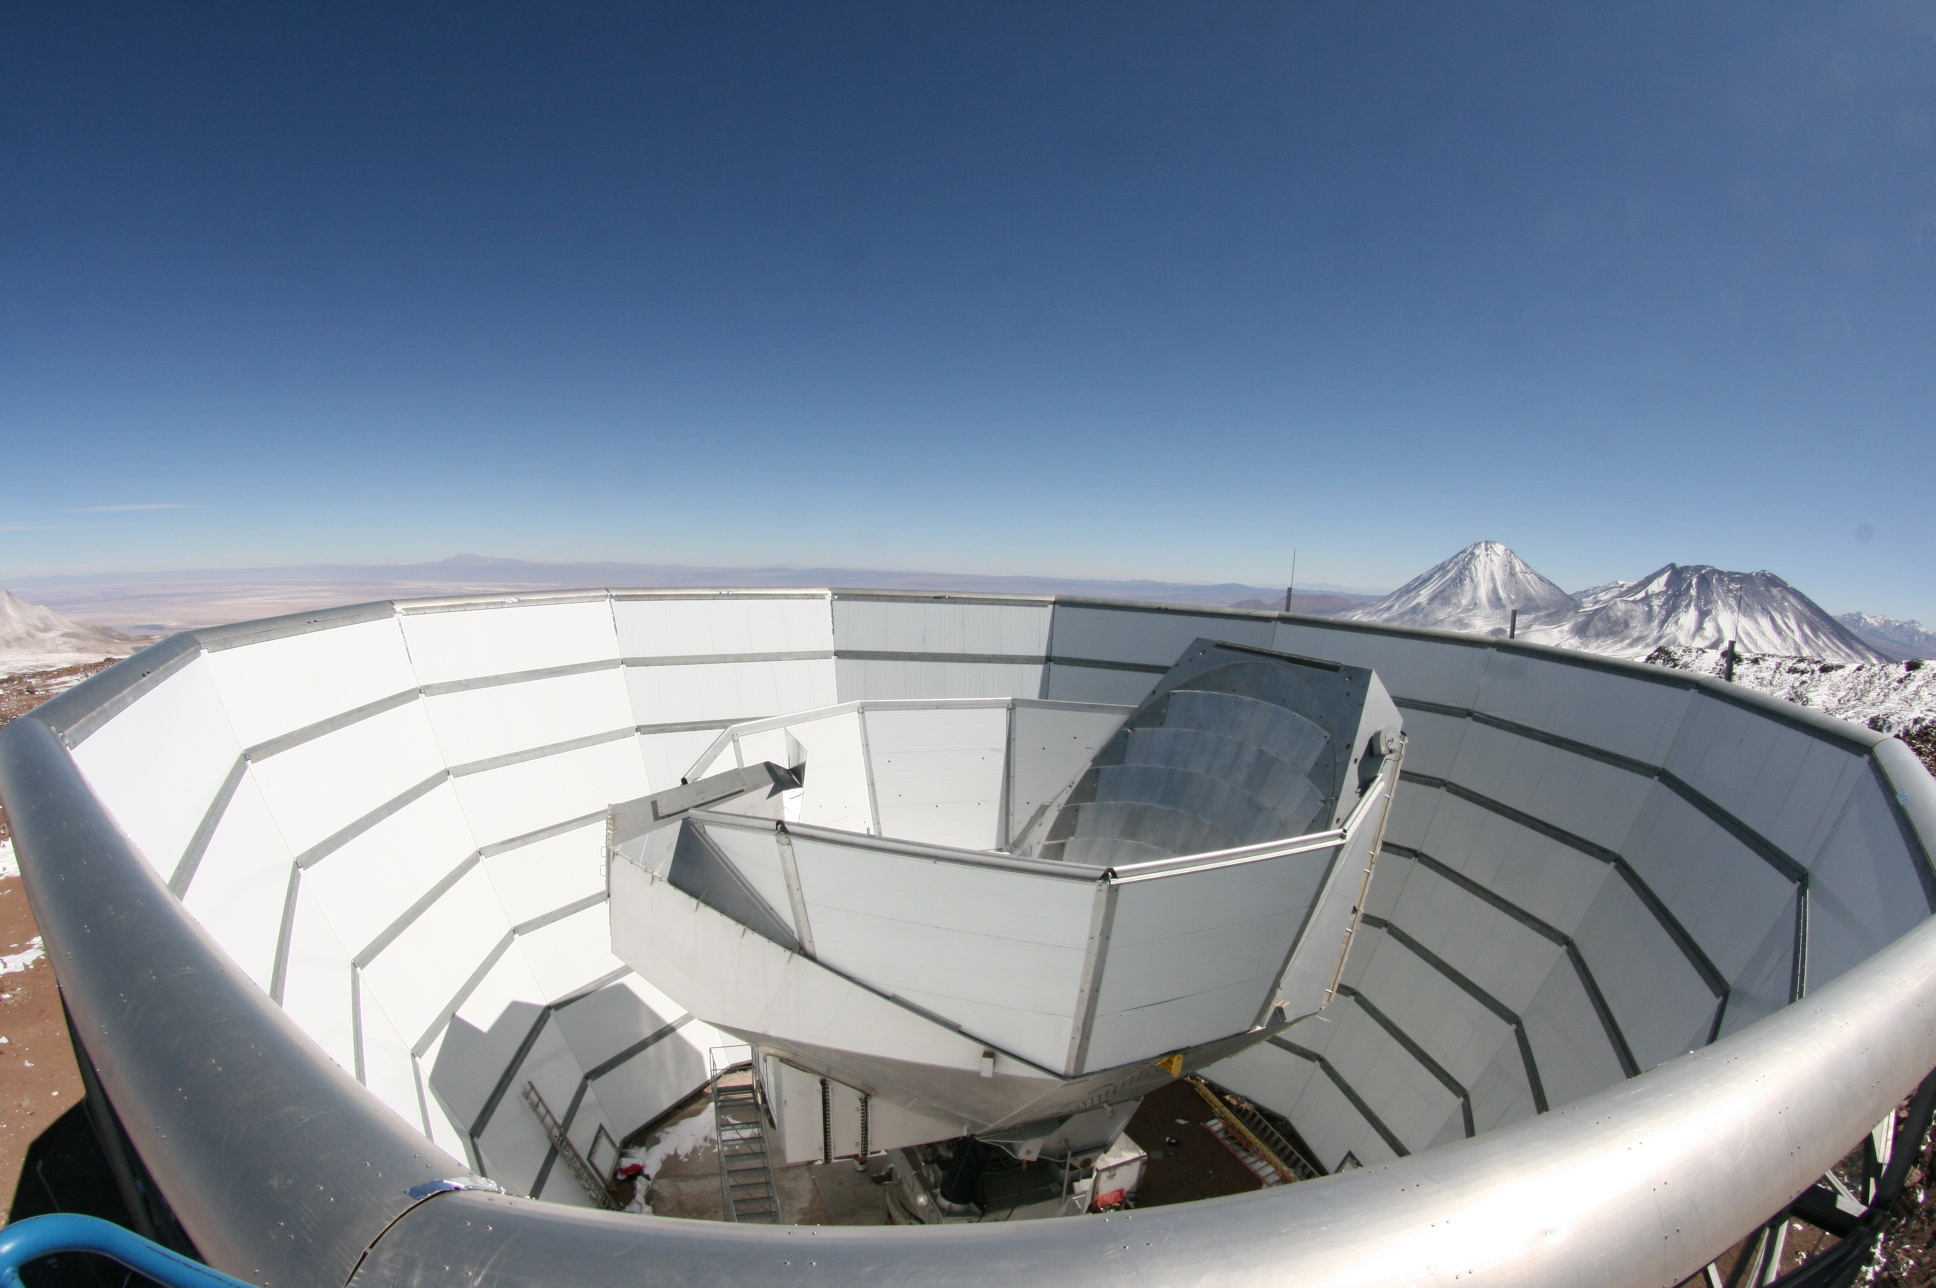
\includegraphics[width = \textwidth]{Figures/act_inst_close.jpeg}
    \caption{The Atacama Cosmology Telescope, surrounded by its outer ground screen. The inner co-moving screen further shields the instrument from any stray-light.  The primary mirror is behind the co-moving screen.}
    \label{fig:act_site}
\end{figure*}

The Atacama Cosmology Telescope (ACT) is a millimeter-wave telescope located on Cerro Toco in the Atacama Desert of Chile at an altitude of 5190\,m.  The full ACT is shown in Figure~\ref{fig:act_site} and the ACT site in Figure~\ref{fig:act_so_site}.  Since its first observations in 2007, the telescope has seen two major instrumentation upgrades: 1) ACTPol and 2) Advanced ACT.  In Chapter~\ref{ch:actbeams}, I present the characterization of the ACT mid-frequency beam and polarization leakage using point-source stacking.

The Advanced ACT, or ``AdvACT", is an upgrade to ACT's three detector arrays and their optics.  Filters and lenses were replaced to operate with the four new multichroic arrays.  This upgrade mapped the CMB in bands from 28\,GHz to 280\,GHz, and mapped approximately half of the sky.  Along with improved angular resolution (1.4' at 150\,GHz and 7.1' at 28\,GHz), the detectors improved polarization and temperature sensitivity due to twice the original number of detectors.
\begin{figure*}[t]
    \centering
    \includegraphics[width=\textwidth]{Figures/Site_Drone_Picture_July_2019.jpeg}
    \caption{The Simons Observatory (SO) and Atacama Cosmology (ACT) site in the Atacama Desert, Chile. The ACT telescope sits within a ground-shield which can be sen in the bottom center.  The outer ground screen protects the telescope from stray light.  The inner co-moving ground-screen further protects the telescope from stray light during observations.}
    \label{fig:act_so_site}
\end{figure*}

Figure~\ref{fig:act_inst} shows the ray-trace of ACT's off-axis Gregorian geometry with two reflectors which guide photons into the receiver cabin; the 6\,m primary is made of 71 adjustable aluminum panels and the 2\,m secondary is made of 11 adjustable aluminum panels~\cite{act_inst}.  The off-axis optical design minimizes scattered power and therefore drastically improves detector sensitivity~\cite{fowler_2007}.  Within the receiver cabin, three cryogenic optics tubes re-image the sky onto the detector arrays~\cite{thornton_2016}.  Light first enters through a 6.4\,mm-thick ultra-high molecular weight polyethylene window, followed by a series of Infra-red (IR) blocking filters at 300\,K, 40\,K, and 4\,K, which reflect out-of-band signal in order to reduce loading on the detectors.  The focal plane of the optics tube is cooled to 100\,mK.   Table~\ref{tab:act} summarizes the optical properties of the ACTPol instrument.

\begin{figure}[t]
    \centering
    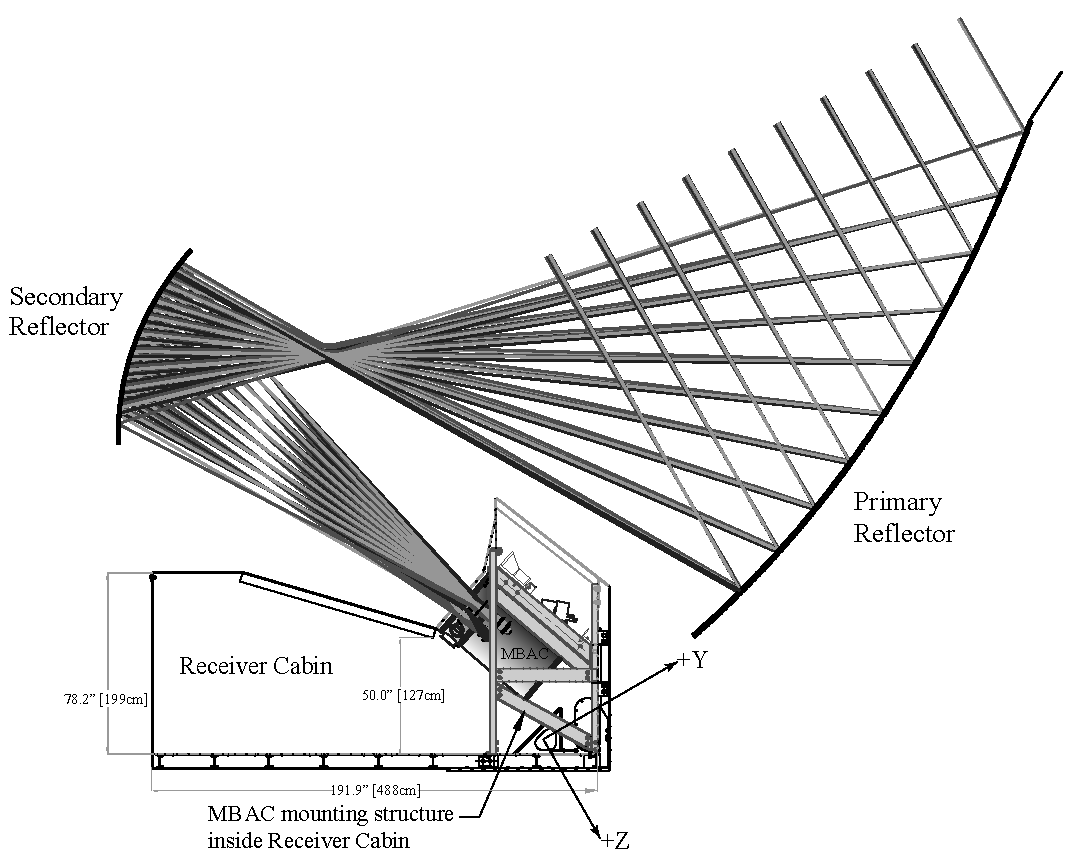
\includegraphics[width = \textwidth]{Figures/act_inst.pdf}
    \caption{Ray-trace diagram of the Atacama Cosmology Telescope~\cite{act_inst}.  The telescope is an off-axis Gregorian with two reflectors: the primary is 6\,m in diameter and the secondary 2\,m.  The rays trace into the Millimeter Bolometer Array Camera (MBAC) cryostat which houses the telescope's detectors.}
    \label{fig:act_inst}
\end{figure}

Since its inception in 2016, AdvACT has achieved many of its ambitious science goals~\cite{2016JLTP184772H}.  With improved sensitivity, ACTPol has measured the intrinsic temperature and polarization anisotropy at high-multipoles, which determines the spectral index of inflation, the primordial helium abundance, and neutrino properties~\cite{10.1117/12.857464}.  Galaxy clusters have also been studied from their Sunyaev-Zel’dovich effect, where CMB photons are scattered by high-energy electrons in the galaxy cluster along the line of sight~\cite{weinberg_cosmo}.  Soon to release its sixth data release (DR6), ACT has turned off observations and scientists will continue to use its groundbreaking data.

\begin{table}[b]
    \centering
    \begin{tabular}{|l|l|l|l|} \hline
        \textbf{ Parameter} & \textbf{MF}   &  \textbf{MF/HF}  & \textbf{HF}  \\ \hline \hline
        Number of Bolometers & 176 & 4430 &1006 \\\hline
        Angular Resolution (arcmin) & $7.1^{\prime}$/$4.8^{\prime}$ & $2.2^{\prime}$/$1.4^{\prime}$ & $0.9^{\prime}$ \\\hline
        Center Frequency (GHz) & 28/41 & 90/150 & 230\\\hline
    \end{tabular} \caption{ACT Key Characteristics~\cite{2016JLTP184772H}.}
    \label{tab:act}
\end{table}
\section{The Simons Observatory}
\begin{figure}[t]
    \centering
    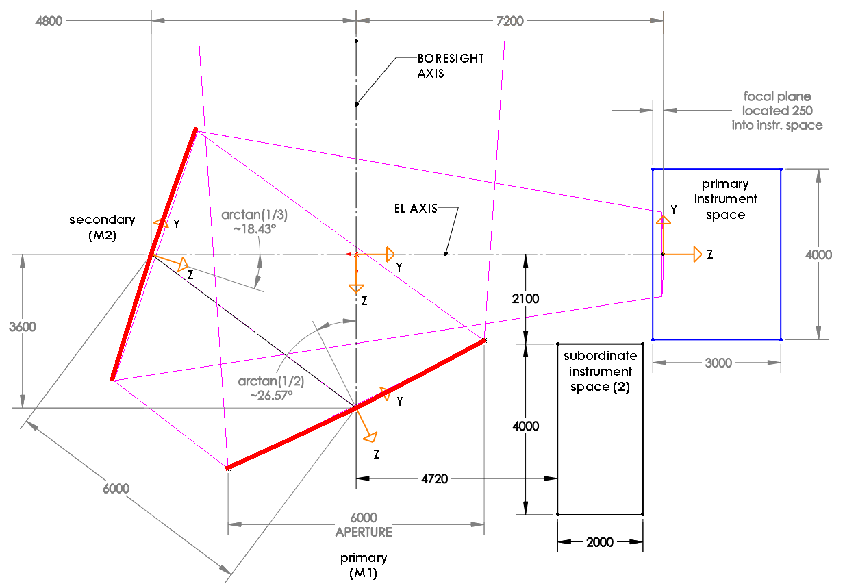
\includegraphics[width = .95\textwidth]{Figures/LAT_rt.pdf}
    \caption{Ray-trace diagram of the Simons Observatory Large Aperture Telescope~\cite{Parshley_2018}.  The telescope is a cross-Dragone with two reflectors, both 6\,m in diameter.  The rays trace into the Large Aperture Telescope Receiver (LATR) cryostat which houses 13 optics tubes.  The optics tubes guide the photons onto the detectors in the focal plane, which are cooled to 100\,mK.}
    \label{fig:so_inst}
\end{figure}
The Simons Observatory (SO) is a series of millimeter-wave telescopes designed to observe the Cosmic Microwave Background (CMB) temperature and polarization signals to an unprecedented sensitivity~\cite{gali18, so19}. With the combination of one Large Aperture Telescope (LAT)~\cite{xu/etal:2020c, zhu18, orlo18, coppi/etal:2018} and three Small Aperture Telescopes (SAT)~\cite{ali20}, the experiment will measure the temperature and polarization anisotropy of the cosmic microwave background with $\sim$\,70,000 background noise limited detectors operating at $\sim$\,100\,mK, covering six frequency bands centered on 27-280\,GHz (Table~\ref{tab:so}).

The resolution of SO will result in a catalog of extragalactic sources, including active galactic nuclei (AGN), dusty star-forming galaxies, and transient sources including Gamma Ray Burst (GRB) afterglows~\cite{so_science}.  SO expects to catalog 10,000-15,000 AGN sources at flux-densities above 7\,mJy~\cite{Tucci_2011}.  The low frequency coverage of SO will complement comparison work with other catalogs (e.g. VLA/VLASS, ASKAP/EMU, MeerKAT/MIGHTEE)~\cite{so_science}.  Dusty star-forming galaxies seen by SO will include local galaxies ($z<0.1)$ and high redshift galaxies (approximately $2<z<4$), and strong lensed galaxies beyond this range~\cite{Marrone_2017}.

\begin{table}[b]
    \centering
    \begin{tabular}{|l|l|l|l|} \hline
        \textbf{ Parameter} &  \textbf{LF} &  \textbf{MF}  &  \textbf{UHF}  \\ \hline \hline
        Number of Bolometers & $>$20,000& $>$20,000& $>$20,000\\\hline
        Angular Resolution (arcmin) & $3.3^{\prime}/3.0^{\prime}$ &$2.10^{\prime}/1.30^{\prime}$&$0.95^{\prime}/0.84^{\prime}$\\\hline
        Center Frequency (GHz) & 27/39 & 90/150 & 220/270\\\hline
    \end{tabular} \caption{SO Key Characteristics~\cite{Gudmundsson:21}.  The number of detectors are split evenly between the three frequency bands.  Note: the LF beam size is estimated by scaling down the MF and UHF beam sizes.}
    \label{tab:so}
\end{table}

\subsection{Large Aperture Telescope}

The Large Aperture Telescope (LAT) will map roughly 40\% of the sky at arcminute resolution~\cite{xu/etal:2020c}.   Figure~\ref{fig:so_inst} shows a cross-section and ray-trace of the LAT.  The primary mirror is 6\,m in diameter and constructed out of 77 individual adjustable panels, while the secondary mirror is 6\,m in diameter and constructed out of 69 adjustable panels \cite{gali18}.

Light from the sky is then reflected into the LAT Receiver (LATR), which houses up to thirteen optics tubes~\cite{Xu_2021}.  The LATR optics tubes re-image the optics onto the detector arrays (three detector arrays per optics tube).  Chapter~\ref{ch:ot_holo} presents radio holography measurements of the LAT optics tube, where I characterize the optical performance of the LAT Receiver optics tube.

\begin{figure*}[ht]
    \centering
    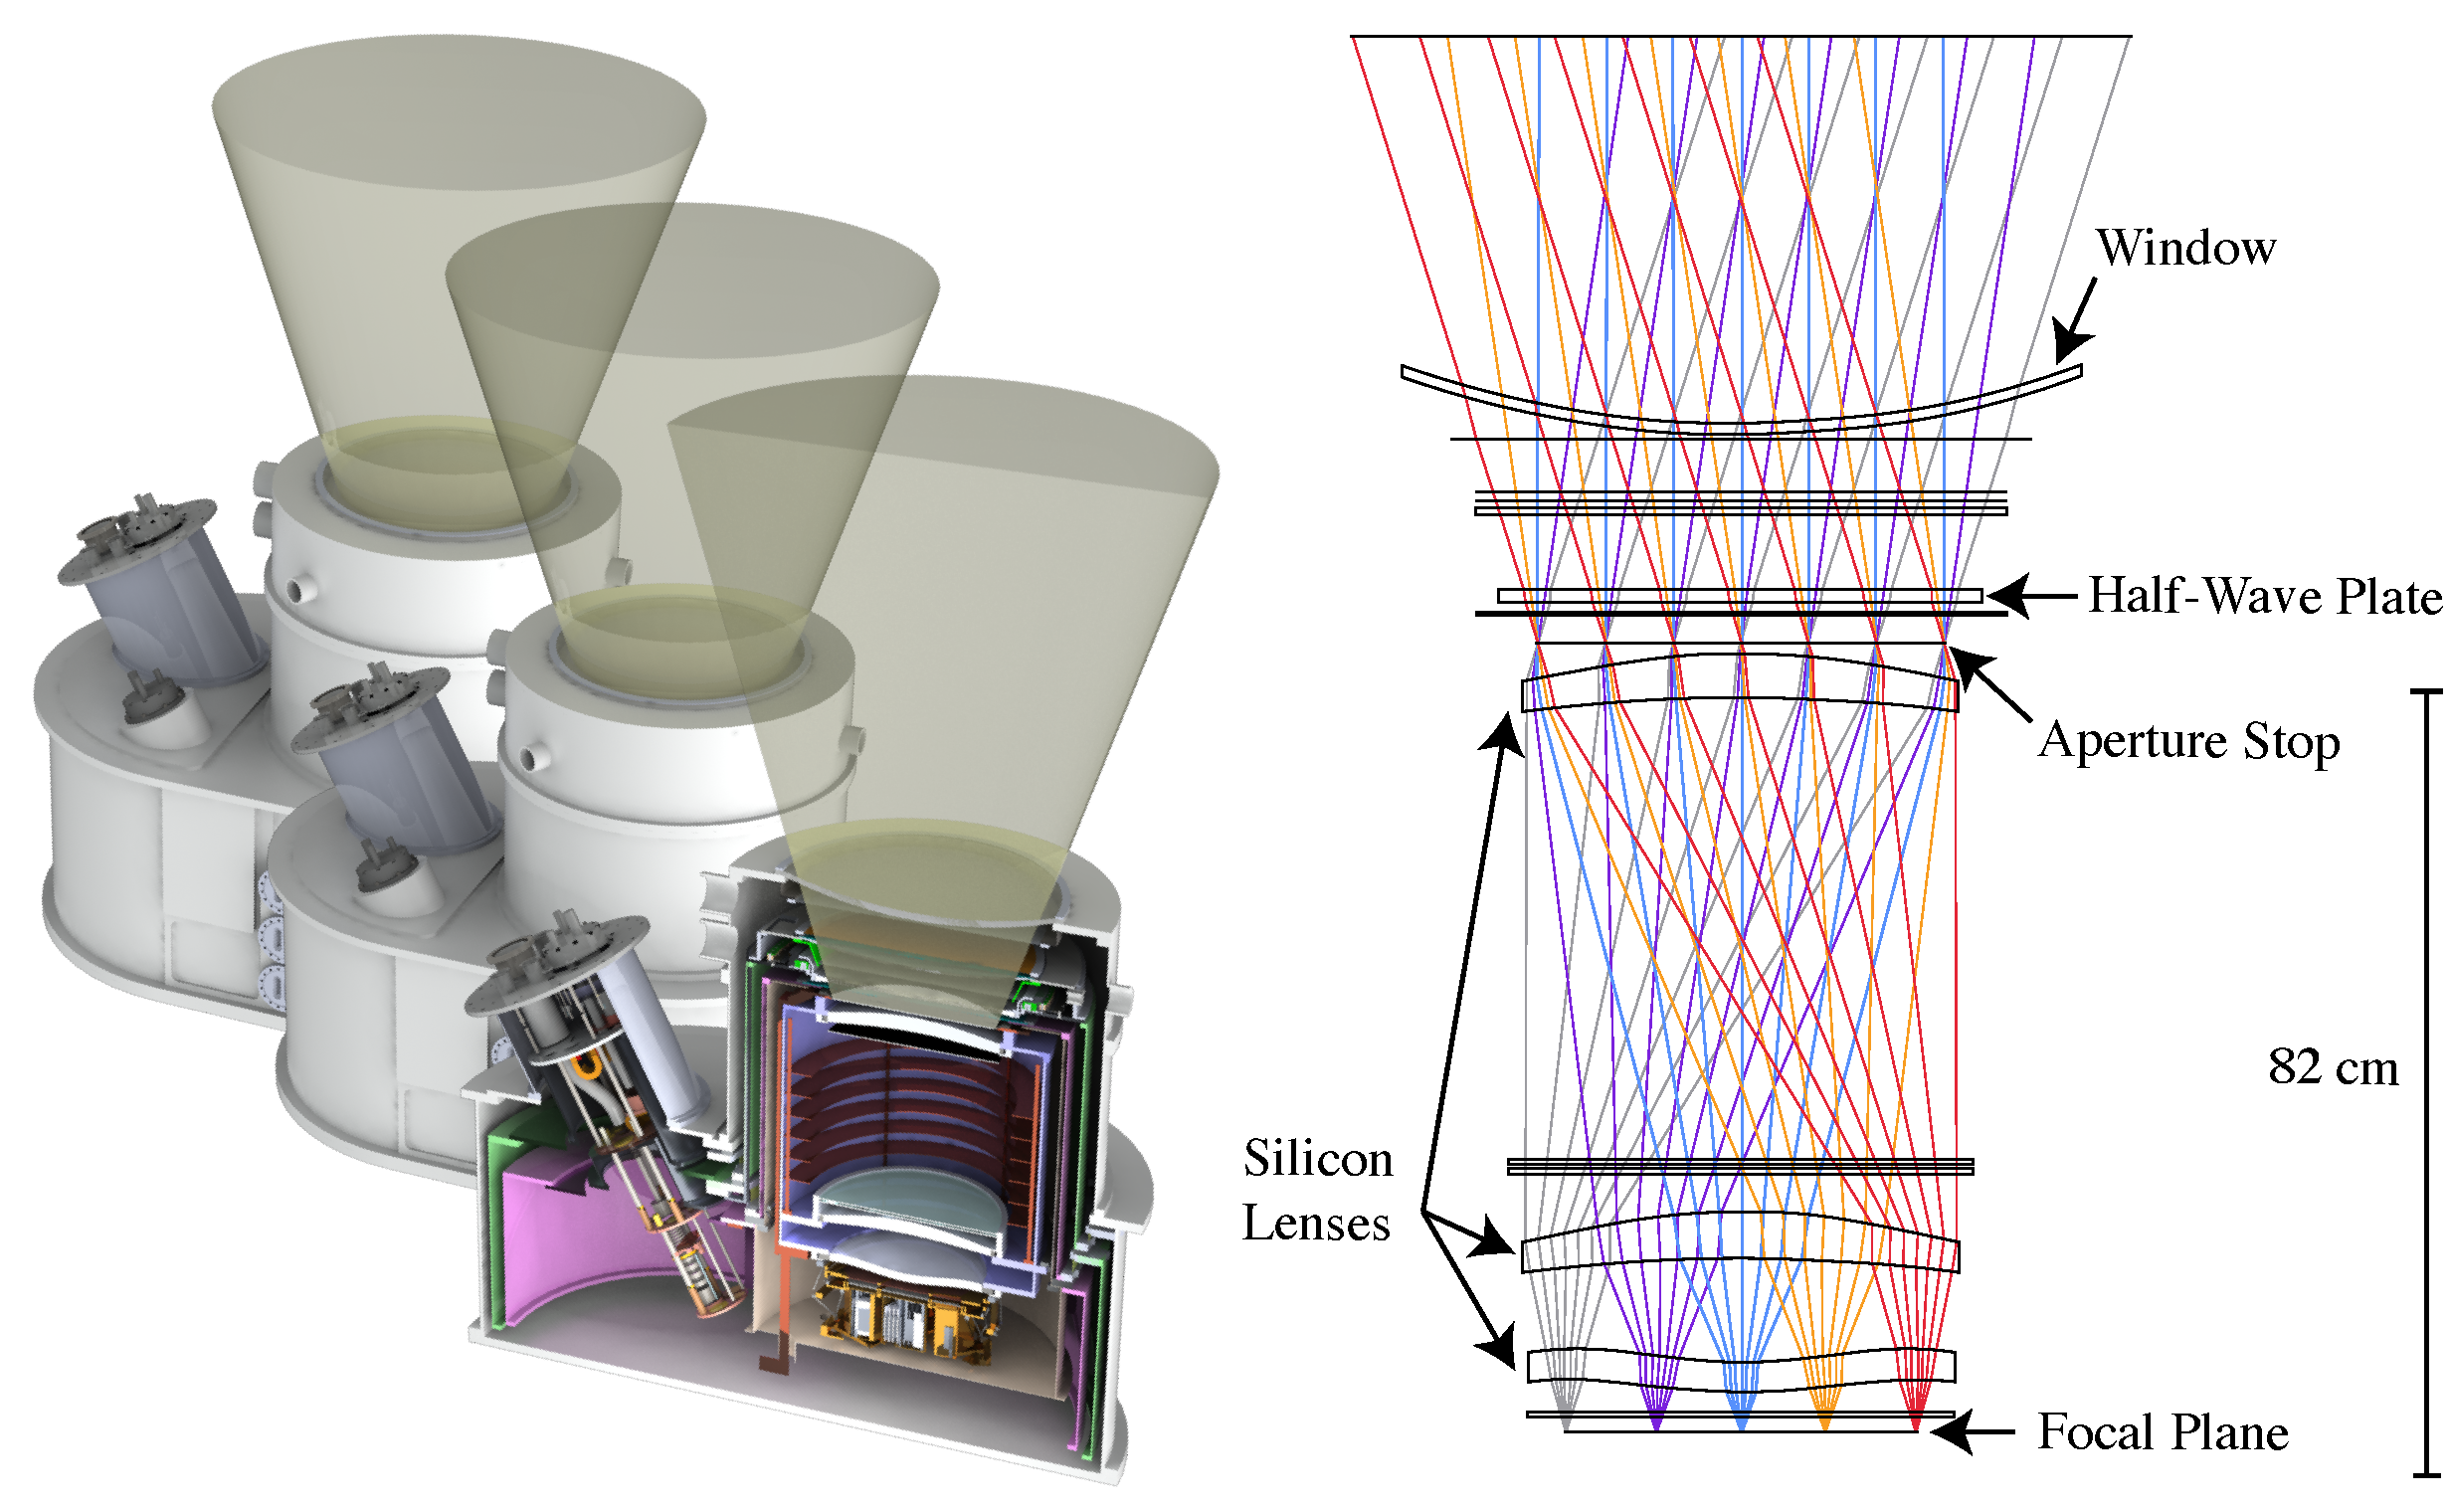
\includegraphics[width = \textwidth]{Figures/SAT3.pdf}
    \caption{Left: Three Small Aperture Telescope cryostats, with the front cross-section showing the inner optics tube.  Right: Ray-trace diagram of the Simons Observatory Small Aperture Telescope~\cite{2020SPIE11445E7LK}.}
    \label{fig:sat3s}
\end{figure*}

\subsection{Small Aperture Telescope}

The Small Aperture Telescope (SAT) optical design is a 0.42\,m diameter refractive telescope (Figure~\ref{fig:sat3s}).  Three SATs will measure the largest angular scales visible from the Atacama Desert.  In total, the three SAT's will hold roughly 30,000 cryogenic detectors, where the SAT is targeting to characterize the CMB on degree angular scales.  In Chapter~\ref{ch:sat_holo}, I present radio holography measurements of the SAT optics tube.

The SAT is a purely refractive telescope.  Figure~\ref{fig:sat3s} shows the ray-trace from the focal plane out the SAT window.  Light enters through a 3\,mm thick ultra-high molecular weight polyethylene hexagonal window with an anti-reflection coating~\cite{zhu18}.  A Cryogenic Half-Wave Plate (CHWP) polarization modulator then reconstructs the polarization of the CMB at 40\,K.  A 1\,K Lyot stop is the first cold optical element, and is followed by the SAT refractor.  Three anti-reflection coated silicon lenses~\cite{Datta:13,golec20} re-image the light onto seven hexagonal detector arrays.   Photons are then coupled onto the detectors by individual feedhorns.  The focal plane of each optics tube houses seven hexagonal detector arrays and are cooled to 100\,mK.

\subsection{The Status of the Simons Observatory}

The Simons Observatory is currently being deployed in the Parque Astronomico located in the Atacama Desert in Chile (Figure~\ref{fig:act_so_site}). The telescope site is situated at an elevation of 5,200 meters near the peak of Cerro Toco at $22 ^\circ$ 57' S, $67^\circ$47' W.  The arid conditions and elevation at the site minimize contamination to millimeter wave signals from water vapor.

Integration and testing occurs in parallel with deployment, as the rollout of the Simons Observatory continues.  In the year to come, SO will begin observations and characterize the CMB with unprecedented sensitivity, with many discoveries of the nature of our universe to come.